\documentclass[11pt,oneside]{article}	%use"amsart"insteadof"article"forAMSLaTeXformat
\usepackage{geometry}		%Seegeometry.pdftolearnthelayoutoptions.Therearelots.
\geometry{letterpaper}		%...ora4paperora5paperor...
%\geometry{landscape}		%Activateforforrotatedpagegeometry
%\usepackage[parfill]{parskip}		%Activatetobeginparagraphswithanemptylineratherthananindent
\usepackage{graphicx}				%Usepdf,png,jpg,orepsßwithpdflatex;useepsinDVImode
								%TeXwillautomaticallyconverteps-->pdfinpdflatex		
\usepackage{amssymb}
\usepackage{hyperref}

%----macros begin---------------------------------------------------------------
\usepackage{color}
\usepackage{amsthm}

\def\conv{\mbox{\textrm{conv}\,}}
\def\aff{\mbox{\textrm{aff}\,}}
\def\E{\mathbb{E}}
\def\R{\mathbb{R}}
\def\Z{\mathbb{Z}}
\def\tex{\TeX}
\def\latex{\LaTeX}
\def\v#1{{\bf #1}}
\def\p#1{{\bf #1}}
\def\T#1{{\bf #1}}

\def\vet#1{{\left(\begin{array}{cccccccccccccccccccc}#1\end{array}\right)}}
\def\mat#1{{\left(\begin{array}{cccccccccccccccccccc}#1\end{array}\right)}}

\def\lin{\mbox{\rm lin}\,}
\def\aff{\mbox{\rm aff}\,}
\def\pos{\mbox{\rm pos}\,}
\def\cone{\mbox{\rm cone}\,}
\def\conv{\mbox{\rm conv}\,}
\newcommand{\homog}[0]{\mbox{\rm homog}\,}
\newcommand{\relint}[0]{\mbox{\rm relint}\,}

%----macros end-----------------------------------------------------------------

\title{Domain mapping with LAR
\footnote{This document is part of the \emph{Linear Algebraic Representation with CoChains} (LAR-CC) framework~\cite{cclar-proj:2013:00}. \today}
}
\author{Alberto Paoluzzi}
%\date{}							%Activatetodisplayagivendateornodate

\begin{document}
\maketitle
\nonstopmode

\begin{abstract}
In this module a first implementation (no optimisations) is done of several \texttt{LAR} operators, reproducing the behaviour of the plasm  \texttt{STRUCT} and \texttt{MAP} primitives, but with better handling of the topology, including the stitching of decomposed (simplicial domains) about their possible sewing. A definition of specialised classes \texttt{Model}, \texttt{Mat} and \texttt{Verts} is also contained in this module, together with the design and the implementation of the \emph{traversal} algorithms for networks of structures.
\end{abstract}

\tableofcontents

%===============================================================================
\section{Introduction}
%===============================================================================

The \texttt{mapper} module, introduced here, aims to provide the tools needed to apply both dimension-independent affine transformations and general simplicial maps to geometric objects and assemblies developed within the LAR scheme. 

For this purpose, a simplicial decomposition of the $[0,1]^d$ hypercube ($d \geq 1$) with any possible \texttt{shape} is firstly given, followed by its scaled version with any  according $\texttt{size}\in\E^d$, being its position vector the mapped image of the point $\mathbf{1}\in\E^d$. A general mapping mechanism is specified, to map any domain decomposition (either simplicial or not) with a given set of ccordinate functions, providing a piecewise-linear approximation of any curved embedding of a $d$-dimensional domain in any $\E^n$ space, with $n \geq d$. 
A suitable function is therefore given to identify corresponding vertices when mapping a domain decomposition of the fundamental polygon of a closed manifold. 

The geometric tools given in this chapter employ a normalised homogeneous representation of vertices of the represented shapes, where the added coordinate is the \emph{last} of the ordered list of vertex coordinates. The homogeneous representation of vertices is used \emph{implicitly}, by inserting the extra coordinate only when needed by the operation at hand, mainly for computing the product of the object's vertices times the matrix of an affine tensor. 

A set of primitive surface and solid shapes is also provided, via the mapping mechanism of a simplicial decomposition of a $d$-dimensional chart. A simplified version of the PLaSM specification of dimension-independent elementary affine transformation is given as well.

The second part of this module is dedicated to the development of a complete framework for the implementation of hierarchical assemblies of shapes and scene graphs, by using the simplest possible set of computing tools. In this case no hierarchical graphs or multigraph are employed, i.e.~no specialised data structures are produced. The ordered list model of hierarchical structures, inherited from PHIGS and PLaSM, is employed in this context. A recursive traversal is used to transform all the component parts of a hierarchical assembly into the reference frame of the first object of the assembly, i.e.~in world coordinates.

%===============================================================================
\section{Piecewise-linear mapping of topological spaces}
%===============================================================================

A very simple but foundational software subsystem is developed in this section, by giving a general mechanism to produce curved maps of topological spaces, via the simplicial decomposition of a chart, i.e.~of a planar embedding of the fundamental polygon of a $d$-dimensional manifold, and the definition of coordinate functions to be applied to its vertices ($0$-cells of the decomposition) to generate an embedding of the manifold.

\subsection{Domain decomposition}
%-------------------------------------------------------------------------------

A simplicial map is a map between simplicial complexes with the property that the images of the vertices of a simplex always span a simplex.  Simplicial maps are thus determined by their effects on vertices, and provide a piecewise-linear approximation of their underlying polyhedra.


\paragraph{Standard and scaled decomposition of unit domain}
The \texttt{larDomain} of given \texttt{shape} is decomposed by \texttt{larSimplexGrid} as an hypercube of dimension $d \equiv\texttt{len(shape)}$, where the \texttt{shape} tuple provides the number or row, columns, pages, etc.~of the decomposition.

%-------------------------------------------------------------------------------
@D Generate a simplicial decomposition ot the $[0,1]^d$ domain
@{""" simplicial decomposition of the unit d-cube """
def larDomain(shape):
	V,CV = larSimplexGrid(shape)
	V = scalePoints(V, [1./d for d in shape])
	return V,CV
@}
%-------------------------------------------------------------------------------

A scaled simplicial decomposition is provided by the second-order  \texttt{larIntervals} function, with \texttt{len(shape)} and \texttt{len(size)} parameters, where the $d$-dimensionale vector \texttt{len(size)} is assumed as the scaling vector to be applied to the point $\mathbf{1}\in\E^d$.

%-------------------------------------------------------------------------------
@D Scaled simplicial decomposition ot the $[0,1]^d$ domain
@{def larIntervals(shape):
	def larIntervals0(size):
		V,CV = larDomain(shape)
		V = scalePoints(V, [scaleFactor for scaleFactor in size])
		return V,CV
	return larIntervals0
@}
%-------------------------------------------------------------------------------

\subsection{Mapping domain vertices}
The second-order texttt{larMap} function is the LAR implementation of the PLaSM primitive \texttt{MAP}.
It is applied to the array \texttt{coordFuncs} of coordinate functions and to the simplicially decomposed  \texttt{domain}, returning an embedded and/or curved \texttt{domain} instance.

%-------------------------------------------------------------------------------
@D Primitive mapping function 
@{def larMap(coordFuncs):
	def larMap0(domain):
		V,CV = domain
		V = TRANS(CONS(coordFuncs)(V))  # plasm CONStruction
		return checkModel((V,CV))
	return larMap0
@}
%-------------------------------------------------------------------------------

\subsection{Identify close or coincident points}

The function \texttt{checkModel}, applied to a \texttt{model} parameter, i.e.~to a (vertices, cells)  pair, returns the model after identification of vertices with coincident or very close position vectors.
The \texttt{checkModel} function works as follows: first a dictionary \texttt{vertDict} is created, with key a suitably approximated position converted into a string by the \texttt{vcode} converter (given in the Appendix), and with value the list of vertex indices with the same (approximated) position. Then, an \texttt{invertedindex} array is created, associating each original vertex index with the new index produced by enumerating the (distinct) keys of the dictionary. Finally, a new list \texttt{CV} of cells is created, by substituting the new vertex indices for the old ones. 

%-------------------------------------------------------------------------------
@D Create a dictionary with key the point location
@{def checkModel(model):
	V,CV = model; n = len(V)
	vertDict = defaultdict(list)
	for k,v in enumerate(V): vertDict[vcode(v)].append(k) 
	points,verts = TRANS(vertDict.items())
	invertedindex = [None]*n
	V = []
	for k,value in enumerate(verts):
		V.append(eval(points[k]))
		for i in value:
			invertedindex[i]=k	
	CV = [[invertedindex[v] for v in cell] for cell in CV]
	# filter out degenerate cells
	CV = [list(set(cell)) for cell in CV if len(set(cell))==len(cell)]
	return V, CV
@}
%-------------------------------------------------------------------------------

\subsection{Embedding or projecting LAR models}
%-------------------------------------------------------------------------------

In order to apply 3D transformations to a two-dimensional LAR model, we must embed it in 3D space, by adding one more coordinate to its vertices. 

\paragraph{Embedding or projecting a geometric model}

This task is performed by the function \texttt{larEmbed} with parameter $k$, that inserts its $d$-dimensional geometric argument in the $x_{d+1}, \ldots, x_{d+k}=0$ subspace of $\E^{d+k}$.
A projection transformation, that removes the last $k$ coordinate of vertices, without changing the object topology, is performed by the function \texttt{larEmbed} with \emph{negative} integer parameter.


%-------------------------------------------------------------------------------
@D Embedding and projecting a geometric model
@{def larEmbed(k):
	def larEmbed0(model):
		V,CV = model
		if k>0:
			V = [v+[0.]*k for v in V] 
		elif k<0:
			V = [v[:-k] for v in V] 
		return V,CV
	return larEmbed0
@}
%-------------------------------------------------------------------------------


%-------------------------------------------------------------------------------
%===============================================================================
\section{Primitive objects}
%===============================================================================

A large number of primitive surfaces or solids is defined in this section, using the \texttt{larMap} mechanism and the coordinate functions of a suitable chart.

%-------------------------------------------------------------------------------
\subsection{1D primitives}
%-------------------------------------------------------------------------------

\paragraph{Circle}
%-------------------------------------------------------------------------------
@D Circle centered in the origin
@{def larCircle(radius=1.):
	def larCircle0(shape=36):
		domain = larIntervals([shape])([2*PI])
		V,CV = domain
		x = lambda V : [radius*COS(p[0]) for p in V]
		y = lambda V : [radius*SIN(p[0]) for p in V]
		return larMap([x,y])(domain)
	return larCircle0
@}
%-------------------------------------------------------------------------------
%-------------------------------------------------------------------------------
\subsection{2D primitives}
%-------------------------------------------------------------------------------
Some useful 2D primitive objects either in $\E^2$ or embedded in $\E^3$ are defined here, including 2D disks and rings, as well as cylindrical, spherical and toroidal surfaces.

\paragraph{Disk}
%-------------------------------------------------------------------------------
@D Disk centered in the origin
@{def larDisk(radius=1.):
	def larDisk0(shape=[36,1]):
		domain = larIntervals(shape)([2*PI,radius])
		V,CV = domain
		x = lambda V : [p[1]*COS(p[0]) for p in V]
		y = lambda V : [p[1]*SIN(p[0]) for p in V]
		return larMap([x,y])(domain)
	return larDisk0
@}
%-------------------------------------------------------------------------------

\paragraph{Ring}
%-------------------------------------------------------------------------------
@D Ring centered in the origin
@{def larRing(params):
	r1,r2 = params
	def larRing0(shape=[36,1]):
		V,CV = larIntervals(shape)([2*PI,r2-r1])
		V = translatePoints(V,[0,r1])
		domain = V,CV
		x = lambda V : [p[1] * COS(p[0]) for p in V]
		y = lambda V : [p[1] * SIN(p[0]) for p in V]
		return larMap([x,y])(domain)
	return larRing0
@}
%-------------------------------------------------------------------------------
\paragraph{Cylinder surface}
%-------------------------------------------------------------------------------
@D Cylinder surface with $z$ axis
@{from scipy.linalg import det
"""
def makeOriented(model):
	V,CV = model
	out = []
	for cell in CV: 
		mat = scipy.array([V[v]+[1] for v in cell]+[[0,0,0,1]])
		if det(mat) < 0.0:
			out.append(cell)
		else:
			out.append([cell[1]]+[cell[0]]+cell[2:])
	return V,out
"""
def larCylinder(params):
	radius,height= params
	def larCylinder0(shape=[36,1]):
		domain = larIntervals(shape)([2*PI,1])
		V,CV = domain
		x = lambda V : [radius*COS(p[0]) for p in V]
		y = lambda V : [radius*SIN(p[0]) for p in V]
		z = lambda V : [height*p[1] for p in V]
		mapping = [x,y,z]
		model = larMap(mapping)(domain)
		# model = makeOriented(model)
		return model
	return larCylinder0
@}
%-------------------------------------------------------------------------------
\paragraph{Spherical surface of given radius}
%-------------------------------------------------------------------------------
@D Spherical surface of given radius
@{def larSphere(radius=1):
	def larSphere0(shape=[18,36]):
		V,CV = larIntervals(shape)([PI,2*PI])
		V = translatePoints(V,[-PI/2,-PI])
		domain = V,CV
		x = lambda V : [radius*COS(p[0])*COS(p[1]) for p in V]
		y = lambda V : [radius*COS(p[0])*SIN(p[1]) for p in V]
		z = lambda V : [radius*SIN(p[0]) for p in V]
		return larMap([x,y,z])(domain)
	return larSphere0
@}
%-------------------------------------------------------------------------------
\paragraph{Toroidal surface}
%-------------------------------------------------------------------------------
@D Toroidal surface of given radiuses
@{def larToroidal(params):
	r,R = params
	def larToroidal0(shape=[24,36]):
		domain = larIntervals(shape)([2*PI,2*PI])
		V,CV = domain
		x = lambda V : [(R + r*COS(p[0])) * COS(p[1]) for p in V]
		y = lambda V : [(R + r*COS(p[0])) * SIN(p[1]) for p in V]
		z = lambda V : [-r * SIN(p[0]) for p in V]
		return larMap([x,y,z])(domain)
	return larToroidal0
@}
%-------------------------------------------------------------------------------
\paragraph{Crown surface}
%-------------------------------------------------------------------------------
@D Half-toroidal surface of given radiuses
@{def larCrown(params):
	r,R = params
	def larCrown0(shape=[24,36]):
		V,CV = larIntervals(shape)([PI,2*PI])
		V = translatePoints(V,[-PI/2,0])
		domain = V,CV
		x = lambda V : [(R + r*COS(p[0])) * COS(p[1]) for p in V]
		y = lambda V : [(R + r*COS(p[0])) * SIN(p[1]) for p in V]
		z = lambda V : [-r * SIN(p[0]) for p in V]
		return larMap([x,y,z])(domain)
	return larCrown0
@}
%-------------------------------------------------------------------------------

%-------------------------------------------------------------------------------
\subsection{3D primitives}
%-------------------------------------------------------------------------------

\paragraph{Ball}
%-------------------------------------------------------------------------------
@D Solid Sphere of given radius
@{def larBall(radius=1):
	def larBall0(shape=[18,36]):
		V,CV = checkModel(larSphere(radius)(shape))
		return V,[range(len(V))]
	return larBall0
@}
%-------------------------------------------------------------------------------

\paragraph{Solid cylinder}
%-------------------------------------------------------------------------------
@D Solid cylinder of given radius and height
@{def larRod(params):
	radius,height= params
	def larRod0(shape=[36,1]):
		V,CV = checkModel(larCylinder(params)(shape))
		return V,[range(len(V))]
	return larRod0
@}
%-------------------------------------------------------------------------------

\paragraph{Solid torus}
%-------------------------------------------------------------------------------
@D Solid torus of given radiuses
@{def larTorus(params):
	r,R = params
	def larTorus0(shape=[24,36,1]):
		domain = larIntervals(shape)([2*PI,2*PI,r])
		V,CV = domain
		x = lambda V : [(R + p[2]*COS(p[0])) * COS(p[1]) for p in V]
		y = lambda V : [(R + p[2]*COS(p[0])) * SIN(p[1]) for p in V]
		z = lambda V : [-p[2] * SIN(p[0]) for p in V]
		return larMap([x,y,z])(domain)
	return larTorus0
@}
%-------------------------------------------------------------------------------

\paragraph{Solid pizza}
%-------------------------------------------------------------------------------
@D Solid pizza of given radiuses
@{def larPizza(params):
	r,R= params
	def larPizza0(shape=[24,36]):
		V,CV = checkModel(larCrown(params)(shape))
		return V,[range(len(V))]
	return larPizza0
@}
%-------------------------------------------------------------------------------
%===============================================================================
\section{Affine transformations}
%===============================================================================
%-------------------------------------------------------------------------------
\subsection{Design decision}
%-------------------------------------------------------------------------------
First we state the general rules that will be satisfied by the matrices used in this module, mainly devoted to apply affine transformations to vertices of models in structure environments:
\begin{enumerate}
\item assume the scipy \texttt{ndarray} as the type of vertices, stored in row-major order;
\item use the last coordinate as the homogeneous coordinate of vertices, but do not store it explicitly;
\item store explicitly the homogeneous coordinate of transformation matrices.
\item use labels '\texttt{verts}' and '\texttt{mat}' to distinguish between vertices and transformation matrices.
\item transformation matrices are dimension-independent, and their dimension is computed as the length of the parameter vector passed to the generating function.
\end{enumerate}


%-------------------------------------------------------------------------------
\subsection{Affine mapping}
%-------------------------------------------------------------------------------

%-------------------------------------------------------------------------------
@D Apply an affine transformation to a LAR model 
@{def larApply(affineMatrix):
	def larApply0(model):
		if isinstance(model,Model):
			V = scipy.dot([v.tolist()+[1.0] for v in model.verts], affineMatrix.T).tolist()
			V = [v[:-1] for v in V]
			CV = copy(model.cells)
			d = copy(model.d)
			return Model((V,CV),d)
		elif isinstance(model,tuple):
			V,CV = model
			V = scipy.dot([v+[1.0] for v in V], affineMatrix.T).tolist()
			return [v[:-1] for v in V],CV
	return larApply0
@}
%-------------------------------------------------------------------------------


%-------------------------------------------------------------------------------
\subsection{Elementary matrices}
%-------------------------------------------------------------------------------
Elementary matrices for affine transformation of vectors in any dimensional vector space are defined here. They include translation, scaling, rotation and shearing. 

\paragraph{Translation}
%-------------------------------------------------------------------------------
@D Translation matrices
@{def t(*args): 
	d = len(args)
	mat = scipy.identity(d+1)
	for k in range(d): 
		mat[k,d] = args[k]
	return mat.view(Mat)
@}
%-------------------------------------------------------------------------------
\paragraph{Scaling}
%-------------------------------------------------------------------------------
@D Scaling matrices
@{def s(*args): 
	d = len(args)
	mat = scipy.identity(d+1)
	for k in range(d): 
		mat[k,k] = args[k]
	return mat.view(Mat)
@}
%-------------------------------------------------------------------------------
\paragraph{Rotation}
%-------------------------------------------------------------------------------
@D Rotation matrices
@{def r(*args): 
	args = list(args)
	n = len(args)
	@< plane rotation (in 2D) @>
	@< space rotation (in 3D) @>
	return mat.view(Mat)
@}
%-------------------------------------------------------------------------------
%-------------------------------------------------------------------------------
@D plane rotation (in 2D)
@{if n == 1: # rotation in 2D
	angle = args[0]; cos = COS(angle); sin = SIN(angle)
	mat = scipy.identity(3)
	mat[0,0] = cos;	mat[0,1] = -sin;
	mat[1,0] = sin;	mat[1,1] = cos;
@}
%-------------------------------------------------------------------------------
%-------------------------------------------------------------------------------
@D space rotation (in 3D)
@{if n == 3: # rotation in 3D
	mat = scipy.identity(4)
	angle = VECTNORM(args); axis = UNITVECT(args)
	cos = COS(angle); sin = SIN(angle)
	@< elementary rotations (in 3D) @>
	@< general rotations (in 3D) @>
@}
%-------------------------------------------------------------------------------
%-------------------------------------------------------------------------------
@D elementary rotations (in 3D)
@{if axis[1]==axis[2]==0.0:	# rotation about x
	mat[1,1] = cos;	mat[1,2] = -sin;
	mat[2,1] = sin;	mat[2,2] = cos;
elif axis[0]==axis[2]==0.0:	# rotation about y
	mat[0,0] = cos;	mat[0,2] = sin;
	mat[2,0] = -sin;	mat[2,2] = cos;
elif axis[0]==axis[1]==0.0:	# rotation about z
	mat[0,0] = cos;	mat[0,1] = -sin;
	mat[1,0] = sin;	mat[1,1] = cos;
@}
%-------------------------------------------------------------------------------
%-------------------------------------------------------------------------------
@D general rotations (in 3D)
@{else:		# general 3D rotation (Rodrigues' rotation formula)	
	I = scipy.identity(3) ; u = axis
	Ux = scipy.array([
		[0,		-u[2], 	 u[1]],
		[u[2],		0, 	-u[0]],
		[-u[1],	 u[0], 		0]])
	UU = scipy.array([
		[u[0]*u[0],	u[0]*u[1],	u[0]*u[2]],
		[u[1]*u[0],	u[1]*u[1],	u[1]*u[2]],
		[u[2]*u[0],	u[2]*u[1],	u[2]*u[2]]])
	mat[:3,:3] = cos*I + sin*Ux + (1.0-cos)*UU
@}


%===============================================================================
\section{Hierarchical complexes}
%===============================================================================
Hierarchical models of complex assemblies are generated by an aggregation
of subassemblies, each one defined in a local coordinate system, and
relocated by affine transformations of coordinates.  This operation
may be repeated hierarchically, with some subassemblies defined by
aggregation of simpler parts, and so on, until one obtains a set of
elementary components, which cannot be further decomposed.

Two main advantages can be found in a hierarchical modeling approach. Each elementary part and each assembly, at every hierarchical level, are defined independently from each other, using a local coordinate frame, suitably chosen to make its definition easier. Furthermore, only one copy of each component is stored in the memory, and may be instanced in different locations and orientations how many times it is needed.

%-------------------------------------------------------------------------------
\subsection{Traversal of hierarchical structures}
%-------------------------------------------------------------------------------

Of course, the main algorithm with hierarchical structures is the \emph{traversal} of the structure network, whose aim is to transform every encountered object from local to global coordinates, where the global coordinates are those of the network root (the only node with indegree zero).

A structure network can be modelled using a directed acyclic multigraph, i.e.~a triple $(N,A,f)$
made by a set $N$ of nodes, a set $A$ of arcs, and a function $f:A \to N^2$ from arcs to ordered pairs of nodes. Conversely that in standard oriented graphs, in this kind of structure more than one oriented arc is allowed between the same pair on nodes.

\begin{figure}[htbp] %  figure placement: here, top, bottom, or page
   \centering
   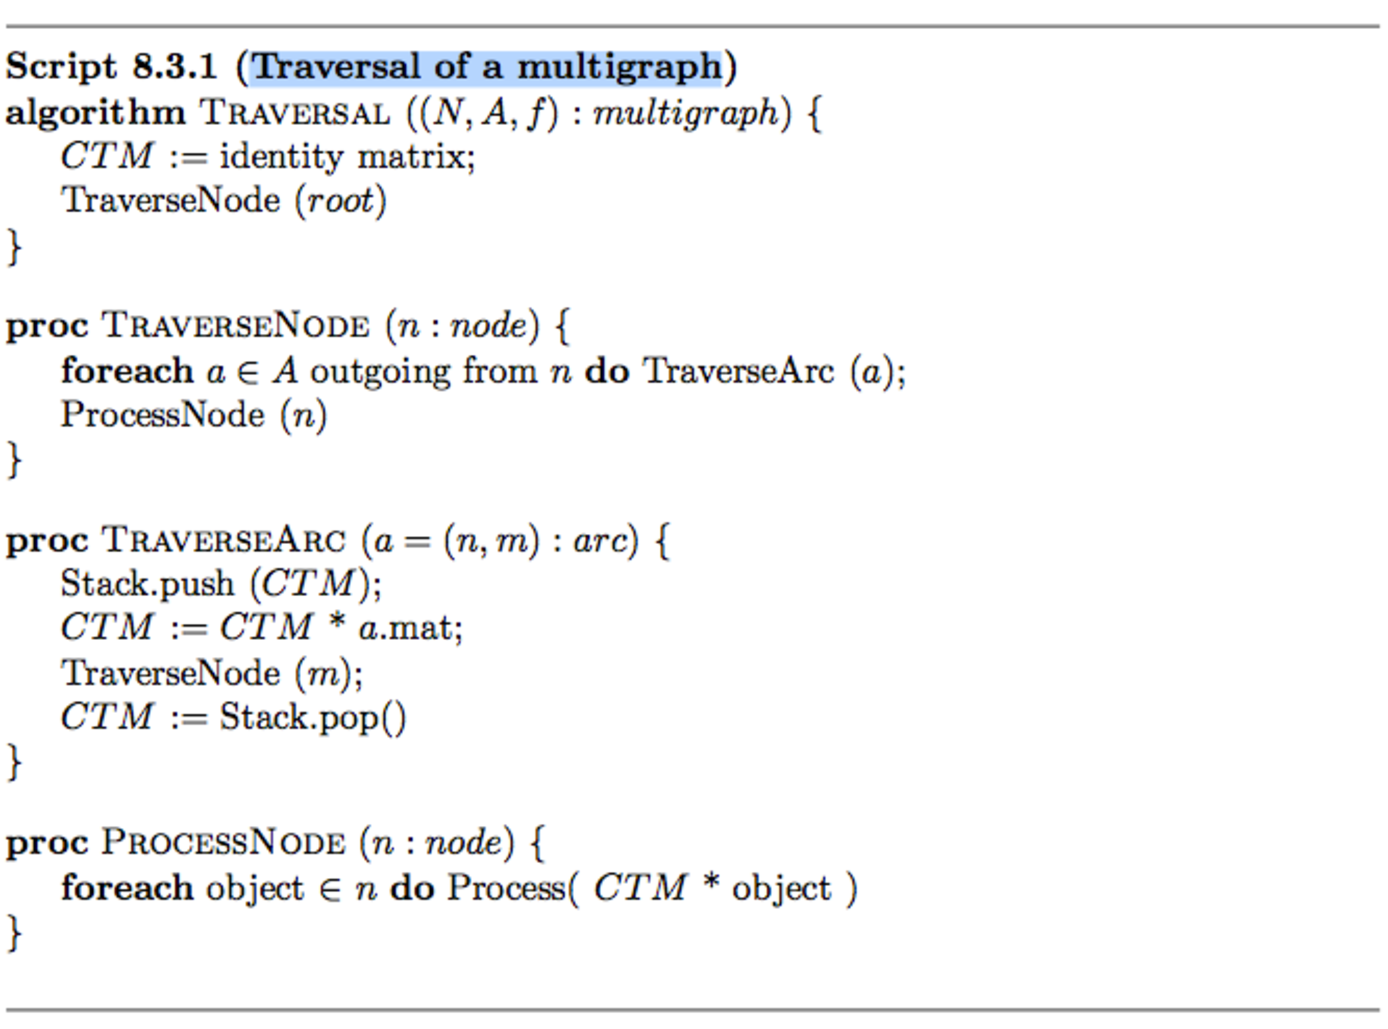
\includegraphics[width=0.8\linewidth]{images/traversal} 
   \caption{Traversal algorithm of an acyclic multigraph.}
   \label{fig:traversal}
\end{figure}

A simple modification of a DFS (Depth First Search) visit of a graph can be used to traverse the structure network This algorithm is given in Figure~\ref{fig:traversal} from~\cite{Paoluzzi2003a}. 

\subsubsection{Traversal of nested lists}

The representation chosen for structure networks with LAR is the serialised one, consisting in ordered sequences (lists) of either (a) LAR models, or (b) affine transformations, or (c) references to other structures, either directly nested within some given structure, or called by reference (name) from within the list.

The aim of a structure network traversal is, of course, to transform every component structure, usually defined in a local coordinate system, into the reference frame of the structure as a whole, normally corresponding with the reference system of the structure's root, called the \emph{world coordinate} system.

\paragraph{The pattern of calls and returned values}

In order to better understand the behaviour of the traversal algorithm, where every transformation is applied to all the following models, --- but only if included in the same structure  (i.e.~list) --- it may be very useful to start with an \emph{algorithm emulation}. In particular, the recursive script below discriminates between three different cases (number, string, or sequence), whereas the actual traversal must do with (a) Models, (b) Matrices, and (c) Structures, respectively.

%-------------------------------------------------------------------------------
@D Emulation of scene multigraph traversal
@{from pyplasm import *
def __traverse(CTM, stack, o):
    for i in range(len(o)):
        if ISNUM(o[i]): print o[i], REVERSE(CTM)
        elif ISSTRING(o[i]): 
            CTM.append(o[i])
        elif ISSEQ(o[i]):
            stack.append(o[i])				# push the stack
            __traverse(CTM, stack, o[i])
            CTM = CTM[:-len(stack)] 		# pop the stack

def algorithm(data):
    CTM,stack = ["I"],[]
    __traverse(CTM, stack, data)  
@}
%-------------------------------------------------------------------------------

Some use example of the above algorithm are provided below. The printout produced at run time is shown from the \texttt{emulation of traversal algorithm} macro.
%-------------------------------------------------------------------------------
@D Examples of multigraph traversal
@{data = [1,"A", 2, 3, "B", [4, "C", 5], [6,"D", "E", 7, 8], 9]  
print algorithm(data)
>>> 1 ['I']
	2 ['A', 'I']
	3 ['A', 'I']
	4 ['B', 'A', 'I']
	5 ['C', 'B', 'A', 'I']
	6 ['B', 'A', 'I']
	7 ['E', 'D', 'B', 'A', 'I']
	8 ['E', 'D', 'B', 'A', 'I']
	9 ['B', 'A', 'I']

data = [1,"A", [2, 3, "B", 4, "C", 5, 6,"D"], "E", 7, 8, 9]  
print algorithm(data)
>>> 1 ['I']
	2 ['A', 'I']
	3 ['A', 'I']
	4 ['B', 'A', 'I']
	5 ['C', 'B', 'A', 'I']
	6 ['C', 'B', 'A', 'I']
	7 ['E', 'A', 'I']
	8 ['E', 'A', 'I']
	9 ['E', 'A', 'I']
@}
%-------------------------------------------------------------------------------
%-------------------------------------------------------------------------------
@D Emulation of traversal algorithm
@{dat = [2, 3, "B", 4, "C", 5, 6,"D"]
print algorithm(dat)
>>> 2 ['I']
	3 ['I']
	4 ['B', 'I']
	5 ['C', 'B', 'I']
	6 ['C', 'B', 'I']
data = [1,"A", dat, "E", 7, 8, 9]
print algorithm(data)
>>> 1 ['I']
	2 ['A', 'I']
	3 ['A', 'I']
	4 ['B', 'A', 'I']
	5 ['C', 'B', 'A', 'I']
	6 ['C', 'B', 'A', 'I']
	7 ['E', 'A', 'I']
	8 ['E', 'A', 'I']
	9 ['E', 'A', 'I']
@}
%-------------------------------------------------------------------------------

\paragraph{Traversal of a scene multigraph}

The previous traversal algorithm is here customised for scene multigraph, where the objects are LAR models, i.e.~pairs of vertices of type '\texttt{Verts} and cells, and where the transformations are matrix transformations of type '\texttt{Mat}'.

\paragraph{Check models for common dimension}
The input list of a call to \texttt{larStruct} primitive is preliminary checked for uniform dimensionality of the enclosed LAR models and transformations. The common dimension \texttt{dim} of models and matrices is returned by the function \texttt{checkStruct}, within the class definition \texttt{Struct} in the module \texttt{lar2psm}. Otherwise, an exception is generated (TODO).

\paragraph{Initialization and call of the algorithm}

The function \texttt{evalStruct} is used to evaluate a structure network, i.e.~to return a \texttt{scene}
list of objects of type \texttt{Model}, all referenced in the world coordinate system. The input variable \texttt{struct} must contain an object of class \texttt{Struct}, i.e.~a reference to an unevaluated structure network. The variable \texttt{dim}  contains the embedding dimension of the structure, i.e.~the number of doordinates of its vertices (normally either 2 or 3), the CTM (Current Transformation Matrix) is initialised to the (homogeneous) identity matrix, and  the \texttt{scene} is returned by calling the \texttt{traverse} algorithm.

%-------------------------------------------------------------------------------
@D Traversal of a scene multigraph
@{""" Traversal of a scene multigraph """
@< Structure traversal algorithm @>
def evalStruct(struct):
    dim = struct.n
    CTM, stack = scipy.identity(dim+1), []
    scene = traversal(CTM, stack, struct) 
    return scene
@}
%-------------------------------------------------------------------------------

\paragraph{Structure traversal algorithm}

The \texttt{traversal} algorithm decides between three different cases, depending on the type of the currently inspected object. If the object is a \texttt{Model} instance, then it applies to it the \texttt{CTM} matrix; else if the object is a \texttt{Mat} instance, then the \texttt{CTM} matrix is updated by (right) product with it; else if the object is a \texttt{Struct} instance, then the \texttt{CTM} is pushed on the stack, initially empty, then the \texttt{traversal} is called (recursion), and finally, at (each) return from recursion, the \texttt{CTM} is recovered by popping the stack.

%-------------------------------------------------------------------------------
@D Structure traversal algorithm 
@{def traversal(CTM, stack, obj, scene=[]):
    for i in range(len(obj)):
        if isinstance(obj[i],Model): 
            scene += [larApply(CTM)(obj[i])]
        elif isinstance(obj[i],Mat): 
            CTM = scipy.dot(CTM, obj[i])
        elif isinstance(obj[i],Struct):
            stack.append(CTM) 
            traversal(CTM, stack, obj[i], scene)
            CTM = stack.pop()
    return scene
@}
%-------------------------------------------------------------------------------


%-------------------------------------------------------------------------------
\subsection{Example}
%-------------------------------------------------------------------------------
Some examples of structures as combinations of LAR models and affine transformations are given in this section. 

\paragraph{Global coordinates}
We start with a simple 2D example of a non-nested list of translated 2D object instances and rotation about the origin.

%-------------------------------------------------------------------------------
@O test/py/mapper/test04.py
@{""" Example of non-nested structure with translation and rotations """
@< Initial import of modules @>
from mapper import *
square = larCuboids([1,1])
table = larApply( t(-.5,-.5) )(square)
chair = larApply( s(.35,.35) )(table)
chair1 = larApply( t(.75, 0) )(chair)
chair2 = larApply( r(PI/2) )(chair1)
chair3 = larApply( r(PI/2) )(chair2)
chair4 = larApply( r(PI/2) )(chair3)
VIEW(SKEL_1(STRUCT(MKPOLS(table)+MKPOLS(chair1)+
				   MKPOLS(chair2)+MKPOLS(chair3)+MKPOLS(chair4))))
@}
%-------------------------------------------------------------------------------

\paragraph{Local coordinates}
A different composition of transformations, from local to global coordinate frames, is used in yje following example.

%-------------------------------------------------------------------------------
@O test/py/mapper/test05.py
@{""" Example of non-nested structure with translation and rotations """
@< Initial import of modules @>
from mapper import *
square = larCuboids([1,1])
square = Model(square,2)
table = larApply( t(-.5,-.5) )(square)
chair = larApply( s(.35,.35) )(table)
chair = larApply( t(.75, 0) )(chair)
struct = Struct([table] + 4*[chair, r(PI/2)])
scene = evalStruct(struct)
VIEW(SKEL_1(STRUCT(CAT(AA(MKPOLS)(scene)))))
@}
%-------------------------------------------------------------------------------

%-------------------------------------------------------------------------------
@O test/py/mapper/test06.py
@{""" Example of nested structures with translation and rotations """
@< Initial import of modules @>
from mapper import *
square = larCuboids([1,1])
square = Model(square,2)
table = larApply( t(-.5,-.5) )(square)
chair = Struct([ t(.75, 0), s(.35,.35), table ])
struct = Struct( [t(2,1)] + [table] + 4*[r(PI/2), chair])
scene = evalStruct(struct)
VIEW(SKEL_1(STRUCT(CAT(AA(MKPOLS)(scene)))))
@}
%-------------------------------------------------------------------------------

%===============================================================================
\section{Computational framework}
%===============================================================================
\subsection{Exporting the library}
%-------------------------------------------------------------------------------
@O lib/py/mapper.py
@{""" Mapping functions and primitive objects """
@< Initial import of modules @>
@< Generate a simplicial decomposition ot the $[0,1]^d$ domain @>
@< Scaled simplicial decomposition ot the $[0,1]^d$ domain @>
@< Create a dictionary with key the point location @>
@< Primitive mapping function @>
@< Basic tests of mapper module @>
@< Circle centered in the origin @>
@< Disk centered in the origin @>
@< Ring centered in the origin @>
@< Spherical surface of given radius @>
@< Cylinder surface with $z$ axis @>
@< Toroidal surface of given radiuses @>
@< Half-toroidal surface of given radiuses @>
@< Solid Sphere of given radius @>
@< Solid cylinder of given radius and height @>
@< Solid torus of given radiuses @>
@< Solid pizza of given radiuses @>
@< Translation matrices @>
@< Scaling matrices @>
@< Rotation matrices @>
@< Embedding and projecting a geometric model @>
@< Apply an affine transformation to a LAR model @>
@< Traversal of a scene multigraph @>
@}
%-------------------------------------------------------------------------------
%===============================================================================
\subsection{Examples}
%===============================================================================

\paragraph{3D rotation about a general axis}

%-------------------------------------------------------------------------------
@O test/py/mapper/test02.py
@{""" General 3D rotation of a toroidal surface """
@< Initial import of modules @>
from mapper import *
model = checkModel(larToroidal([0.2,1])())
a,b,c = SCALARVECTPROD([PI/2,UNITVECT([1,1,0]) ])
model = larApply(r(a,b,c))(model)
VIEW(STRUCT(MKPOLS(model)))
@}
%-------------------------------------------------------------------------------


\paragraph{3D rotation of a 2D circle}

%-------------------------------------------------------------------------------
@O test/py/mapper/test03.py
@{""" Elementary 3D rotation of a 2D circle """
@< Initial import of modules @>
from mapper import *
model = checkModel(larCircle(1)())
model = larEmbed(1)(model)
model = larApply(r(PI/2,0,0))(model)
VIEW(STRUCT(MKPOLS(model)))
@}
%-------------------------------------------------------------------------------




%===============================================================================
\subsection{Tests}
%===============================================================================

	
%-------------------------------------------------------------------------------
@D Basic tests of mapper module
@{if __name__=="__main__":
	V,EV = larDomain([5])
	VIEW(EXPLODE(1.5,1.5,1.5)(MKPOLS((V,EV))))
	V,EV = larIntervals([24])([2*PI])
	VIEW(EXPLODE(1.5,1.5,1.5)(MKPOLS((V,EV))))
		
	V,FV = larDomain([5,3])
	VIEW(EXPLODE(1.5,1.5,1.5)(MKPOLS((V,FV))))
	V,FV = larIntervals([36,3])([2*PI,1.])
	VIEW(EXPLODE(1.5,1.5,1.5)(MKPOLS((V,FV))))
		
	V,CV = larDomain([5,3,1])
	VIEW(EXPLODE(1.5,1.5,1.5)(MKPOLS((V,CV))))
	V,CV = larIntervals([36,2,3])([2*PI,1.,1.])
	VIEW(EXPLODE(1.5,1.5,1.5)(MKPOLS((V,CV))))
@}
%-------------------------------------------------------------------------------

\paragraph{Circumference of unit radius}

%-------------------------------------------------------------------------------
@O test/py/mapper/test01.py
@{""" Circumference of unit radius """
@< Initial import of modules @>
from mapper import *
model = checkModel(larCircle(1)())
VIEW(EXPLODE(1.2,1.2,1.2)(MKPOLS(model)))
model = checkModel(larDisk(1)([36,4]))
VIEW(EXPLODE(1.2,1.2,1.2)(MKPOLS(model)))
model = checkModel(larRing([.9, 1.])([36,2]))
VIEW(EXPLODE(1.2,1.2,1.2)(MKPOLS(model)))
model = checkModel(larCylinder([.5,2.])([32,1]))
VIEW(STRUCT(MKPOLS(model)))
model = checkModel(larSphere(1)())
VIEW(STRUCT(MKPOLS(model)))
model = larBall(1)()
VIEW(STRUCT(MKPOLS(model)))
model = larRod([.25,2.])([32,1])
VIEW(STRUCT(MKPOLS(model)))
model = checkModel(larToroidal([0.5,1])())
VIEW(STRUCT(MKPOLS(model)))
model = checkModel(larCrown([0.125,1])([8,48]))
VIEW(STRUCT(MKPOLS(model)))
model = larPizza([0.05,1])([8,48])
VIEW(STRUCT(MKPOLS(model)))
model = checkModel(larTorus([0.5,1])())
VIEW(STRUCT(MKPOLS(model)))
@}
%-------------------------------------------------------------------------------


%===============================================================================
\appendix
\section{Utility functions}
%===============================================================================

%-------------------------------------------------------------------------------
@D Initial import of modules
@{from pyplasm import *
from scipy import *
import os,sys

""" import modules from larcc/lib """
sys.path.insert(0, 'lib/py/')
@< Import the module @(lar2psm@) @>
@< Import the module @(simplexn@) @>
@< Import the module @(larcc@) @>
@< Import the module @(largrid@) @>
@< Import the module @(boolean2@) @>
@}
%-------------------------------------------------------------------------------

%-------------------------------------------------------------------------------
@D Import the module
@{import @1
from @1 import *
@}
%-------------------------------------------------------------------------------


\subsection{Numeric utilities}

A small set of utilityy functions is used to transform a point representation as array of coordinates into a string of fixed format to be used as point key into python dictionaries.

%------------------------------------------------------------------
@D Symbolic utility to represent points as strings
@{""" TODO: use package Decimal (http://docs.python.org/2/library/decimal.html) """
ROUND_ZERO = 1E-07
def round_or_zero (x,prec=7):
	"""
	Decision procedure to approximate a small number to zero.
	Return either the input number or zero.
	"""
	def myround(x):
		return eval(('%.'+str(prec)+'f') % round(x,prec))
	xx = myround(x)
	if abs(xx) < ROUND_ZERO: return 0.0
	else: return xx

def prepKey (args): return "["+", ".join(args)+"]"

def fixedPrec(value):
	if abs(value - int(value))<ROUND_ZERO: value = int(value)
	out = ('%0.7f'% value).rstrip('0')
	if out == '-0.': out = '0.'
	return out
	
def vcode (vect): 
	"""
	To generate a string representation of a number array.
	Used to generate the vertex keys in PointSet dictionary, and other similar operations.
	"""
	return prepKey(AA(fixedPrec)(vect))
@}
%------------------------------------------------------------------


\bibliographystyle{amsalpha}
\bibliography{mapper}

\end{document}
